%% ICNDEMAC-2027 -- Track 1: Nano-Materials for Advanced Devices (nano-photonics)
%% IEEE conference paper (IEEEtran). Build with pdflatex (x2), or Overleaf.
\documentclass[conference]{IEEEtran}
\IEEEoverridecommandlockouts

\usepackage{cite}
\usepackage{amsmath,amssymb,amsfonts}
\usepackage{graphicx}
\usepackage{booktabs}
\usepackage{textcomp}
\usepackage{xcolor}
\usepackage[hidelinks]{hyperref}

\graphicspath{{figures/}}

\begin{document}

\title{Finite-Element Drift-Diffusion Modelling of Direct-Gap\\
III--V Light-Emitting Diodes: Wavelength Tuning and\\
Double-Heterostructure Efficiency in Nano-Photonic Emitters}

\author{%
\IEEEauthorblockN{Author One\IEEEauthorrefmark{1}, Author Two\IEEEauthorrefmark{2}}
\IEEEauthorblockA{\textit{Department of Electronics and Communication Engineering}\\
\textit{Affiliation, City, Country}\\
\IEEEauthorrefmark{1}email@domain \quad \IEEEauthorrefmark{2}email@domain}
}

\maketitle

\begin{abstract}
Direct-gap III--V semiconductors are the material basis of nano-photonic
light emitters, and their design---band-gap engineering for a target wavelength
and heterostructure engineering for efficiency---requires a device simulator that
couples carrier transport to radiative recombination and optical output. We
present an open-source, two-dimensional finite-element drift-diffusion (DD) solver
that adds a bimolecular (radiative) recombination channel and an optical
post-processor reporting the internal quantum efficiency (IQE), emission
wavelength and optical power, together with heterojunction band offsets
(Anderson's rule), a self-consistent Schr\"odinger--Poisson quantum correction,
and Fermi--Dirac statistics for degenerate cladding. For a GaAs homojunction LED
the solver reproduces the analytic built-in potential ($1.151$~V, numeric $=$
analytic) and an emission wavelength of $873$~nm set by the $1.42$~eV gap, with a
peak IQE of $0.53$. Sweeping the active material tunes the emission from the
near-infrared (GaAs, $873$~nm) through the red (Al\textsubscript{0.3}Ga\textsubscript{0.7}As,
$689$~nm) to the ultraviolet (GaN, $366$~nm), following the material band gap. A
GaAs/AlGaAs double-heterostructure (DH) LED confines both carrier types in the
narrow-gap active region; the resulting overlap raises the peak IQE from $0.53$
(homojunction) to $0.90$, quantifying the classic DH efficiency advantage on a
single, self-consistent transport model. The tool provides a compact, physically
transparent platform for the design of nano-scale direct-gap emitters.
\end{abstract}

\begin{IEEEkeywords}
Light-emitting diode, radiative recombination, direct-gap semiconductor,
double heterostructure, internal quantum efficiency, drift-diffusion,
finite-element method, GaAs, AlGaAs, GaN, nano-photonics.
\end{IEEEkeywords}

\section{Introduction}
\IEEEPARstart{L}{ight-emitting} diodes built from direct-gap III--V
semiconductors are central to solid-state lighting, displays, optical
interconnect and sensing, and their nanoscale active regions---thin double
heterostructures, quantum wells---are the emerging materials of advanced
photonic devices~\cite{schubert}. Two engineering levers dominate their design:
the choice of active material, which sets the emission wavelength through the band
gap, and the heterostructure, which confines injected carriers to raise the
radiative efficiency~\cite{kroemer,caseypanish}. Predictive design therefore needs
a device model that couples electrical transport to the radiative process and to
the optical output.

The drift-diffusion (DD) framework~\cite{selberherr} is the standard basis for such
modelling. To describe an emitter it must be augmented with (i) a radiative
(bimolecular) recombination channel that both consumes carriers and produces
photons, (ii) heterojunction band-edge offsets so that a narrow-gap active region
clad by a wider-gap material actually confines carriers, and (iii)---for the thin,
degenerately-doped layers of a real device---quantum-confinement and
Fermi--Dirac corrections. This paper presents a compact, open-source
finite-element solver that integrates all of these, and uses it to characterise
wavelength tuning across III--V materials and the efficiency gain of a
double-heterostructure emitter.

\textit{Contributions.} (i) A 2-D finite-element DD solver with a bimolecular
radiative channel and an optical post-processor (IQE, wavelength, optical power)
that is current-consistent by construction; (ii) heterojunction electrostatics,
a self-consistent Schr\"odinger--Poisson correction and Fermi--Dirac statistics on
the same mesh; (iii) validated GaAs LED characteristics; (iv) demonstrations of
material-tuned emission from the near-infrared to the ultraviolet and of the
double-heterostructure efficiency advantage.

\section{Device Model}

\subsection{Drift-diffusion core}
The steady state is solved in the normalised quasi-Fermi-potential variables
$u=\psi/V_T$, $v=\phi_n/V_T$, $w=\phi_p/V_T$ (De Mari scaling~\cite{demari}), with
$n=n_ie^{\,u-v}$, $p=n_ie^{\,w-u}$. Poisson's equation and the two carrier
continuity equations are discretised with linear (P1) triangular finite elements
and assembled into a $3N\times3N$ system solved by a fully-coupled damped Newton
method using an exact analytic Jacobian. Terminal currents are extracted as the
sum of the natural continuity residuals over a contact's nodes, which is
conservative by construction.

\subsection{Radiative recombination and optical output}
The light-emitting mechanism of a direct-gap diode is radiative (bimolecular)
recombination, added as a net-recombination term
\begin{equation}
R_{\mathrm{rad}}=B\,(np-n_i^2),
\end{equation}
where $B$ (m\textsuperscript{3}\,s\textsuperscript{-1}) is the material radiative
coefficient. Because of the $(np-n_i^2)$ prefactor the rate vanishes at
equilibrium and leaves it unchanged; its exact derivatives
$\partial R/\partial n=Bp$, $\partial R/\partial p=Bn$ enter the analytic Jacobian,
preserving quadratic convergence. Shockley--Read--Hall and Auger channels are
included as competing non-radiative paths. After a converged forward-bias solve
the optical post-processor integrates the radiative rate over the device (on the
same quadrature and corrected densities used in the assembly) and reports
\begin{align}
I_{\mathrm{rad}} &= q\,R_{\mathrm{rad}}, &
\mathrm{IQE} &= \frac{R_{\mathrm{rad}}}{R_{\mathrm{rad}}+R_{\mathrm{SRH}}+R_{\mathrm{Auger}}},\\
E_{\mathrm{ph}} &= E_g^{\mathrm{active}}, &
\lambda &= \frac{hc}{E_{\mathrm{ph}}}, \quad P_{\mathrm{opt}}=R_{\mathrm{rad}}E_{\mathrm{ph}}.
\end{align}
By construction $q R_{\mathrm{rad}}$ equals the radiative part of the terminal
current, so the electrical and optical outputs are mutually consistent. The
radiative coefficient is significant only in direct-gap materials; the bundled
direct-gap files (GaAs, AlGaAs, GaN) carry representative $300$~K values, and a
guardrail warns if radiative emission is requested on an indirect material.

\subsection{Heterojunction, quantum and Fermi--Dirac corrections}
Multi-material devices are solved with a heterojunction electrostatics core:
position-dependent permittivity and mobility, and band-edge offsets
$\Delta E_c,\Delta E_v$ from Anderson's electron-affinity rule that appear as fixed
additive shifts in the carrier-density exponents. A narrow-gap active region clad
by a wider-gap material therefore presents potential barriers that confine both
carrier types. For thin bodies a self-consistent Schr\"odinger--Poisson correction
quantises the transverse states into subbands and enters transport as a
charge-conserving additive quantum potential; for degenerately-doped cladding,
Fermi--Dirac statistics enter as a degeneracy shift refreshed by the same outer
self-consistency loop. All corrections vanish in their respective non-degenerate,
bulk limits, recovering the classical Boltzmann solver exactly.

\section{Results and Discussion}

\subsection{GaAs LED: validation and characteristics}
A GaAs $p$--$n$ homojunction ($N_A=N_D=10^{16}\,\mathrm{cm^{-3}}$, $E_g=1.42$~eV,
$n_i=2.15\times10^6\,\mathrm{cm^{-3}}$, $B=2\times10^{-16}\,\mathrm{m^3 s^{-1}}$)
gives a numerical built-in potential of $1.151$~V, matching the analytic
$V_{bi}=V_T\ln(N_AN_D/n_i^2)=1.151$~V. Fig.~\ref{fig:gaasiv} shows the forward
$I$--$V$ together with the radiative component $I_{\mathrm{rad}}=qR_{\mathrm{rad}}$;
at $1.3$~V the device carries $53.7$~$\mu$A total with $1.68$~$\mu$A radiative and
$2.4$~$\mu$W of optical output. The emission wavelength is $873$~nm
($E_{\mathrm{ph}}=1.42$~eV), the expected near-infrared line of GaAs. The internal
quantum efficiency (Fig.~\ref{fig:gaasiqe}) rises with injection as the
bimolecular rate ($\propto np$) overtakes the SRH channel, reaching a peak of
$0.53$.

\begin{figure}[!t]
\centering
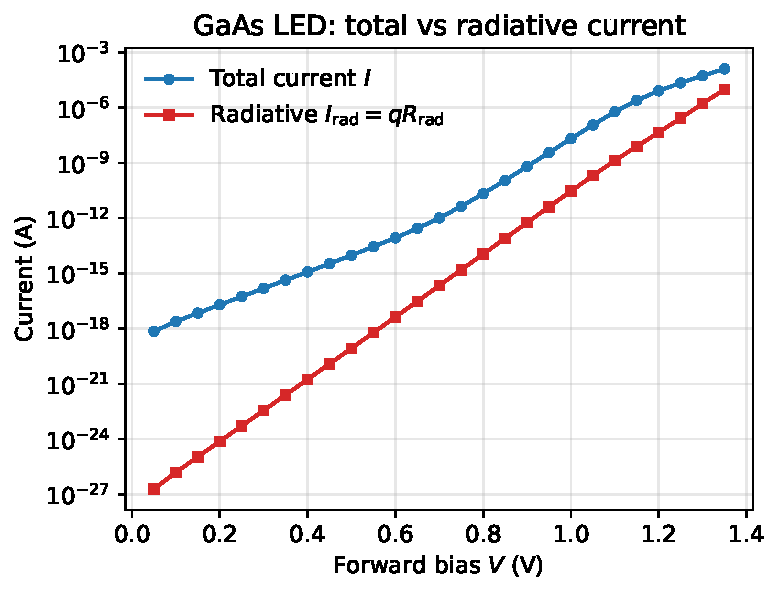
\includegraphics[width=\columnwidth]{fig_gaas_iv.pdf}
\caption{GaAs LED forward characteristics: total terminal current and its
radiative part $I_{\mathrm{rad}}=qR_{\mathrm{rad}}$, which are consistent by
construction.}
\label{fig:gaasiv}
\end{figure}

\begin{figure}[!t]
\centering
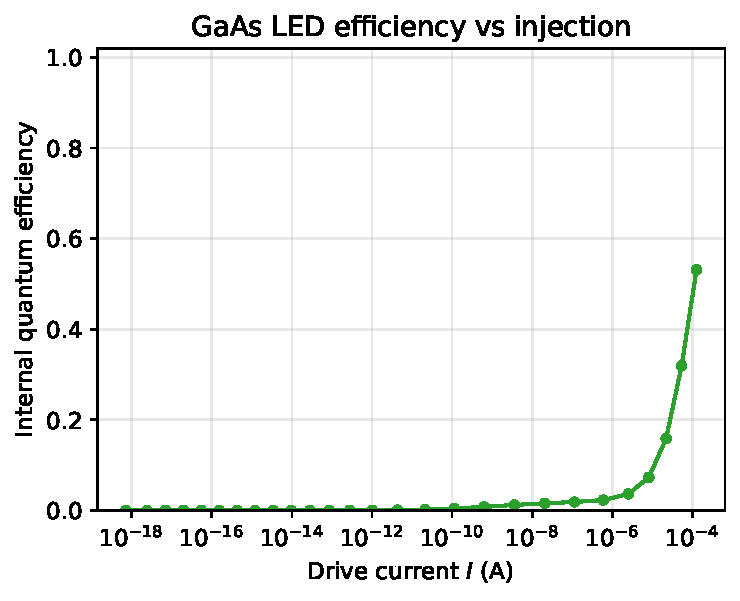
\includegraphics[width=\columnwidth]{fig_gaas_iqe.pdf}
\caption{GaAs LED internal quantum efficiency versus drive current. IQE rises as
the bimolecular radiative rate overtakes non-radiative SRH recombination, peaking
at $0.53$.}
\label{fig:gaasiqe}
\end{figure}

\subsection{Material-tuned emission}
Keeping the device geometry fixed and changing only the active material tunes the
emission wavelength through the band gap (Fig.~\ref{fig:tuning},
Table~\ref{tab:tuning}): GaAs emits at $873$~nm (near-infrared),
Al\textsubscript{0.3}Ga\textsubscript{0.7}As at $689$~nm (red), and GaN at
$366$~nm (ultraviolet). The solver converges the full electrical problem for each
material---spanning intrinsic densities from $n_i\sim10^6\,\mathrm{cm^{-3}}$ (GaAs)
down to the extremely small $n_i$ of wide-gap GaN---and returns the emission line
directly from the active-region gap. This spans the technologically important
range from optical-communication wavelengths to visible and UV emitters on a
single, consistent model.

\begin{table}[!t]
\caption{Material-tuned emission (fixed geometry, $N_A=N_D=10^{16}$~cm$^{-3}$)}
\label{tab:tuning}
\centering
\begin{tabular}{lccl}
\toprule
active material & $E_g$ (eV) & $\lambda$ (nm) & spectral band\\
\midrule
GaAs & 1.42 & 873 & near-infrared\\
Al\textsubscript{0.3}Ga\textsubscript{0.7}As & 1.80 & 689 & red (visible)\\
GaN  & 3.39 & 366 & ultraviolet\\
\bottomrule
\end{tabular}
\end{table}

\begin{figure}[!t]
\centering
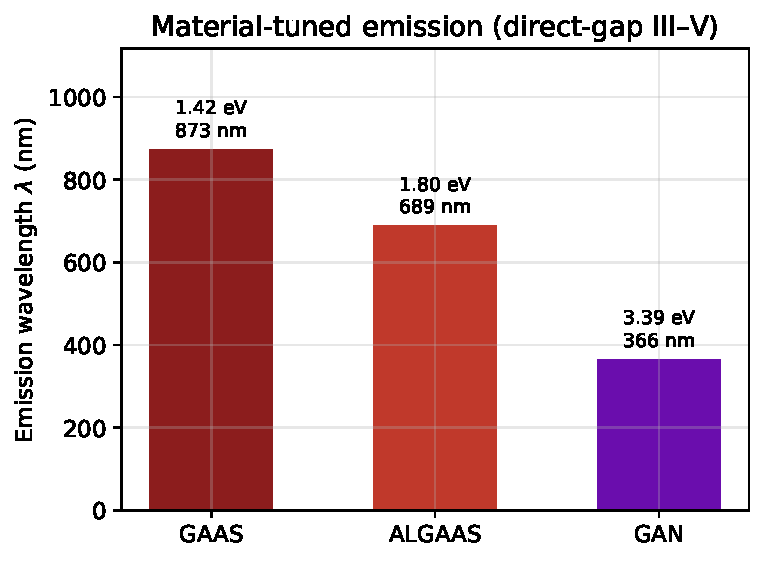
\includegraphics[width=\columnwidth]{fig_wavelength_tuning.pdf}
\caption{Emission wavelength for three direct-gap III--V active materials,
labelled with the band gap. The wavelength follows $\lambda=hc/E_g$, spanning
the near-infrared to the ultraviolet.}
\label{fig:tuning}
\end{figure}

\subsection{Double-heterostructure efficiency advantage}
Fig.~\ref{fig:dhconf} shows the carrier densities along the transport direction of
a GaAs/AlGaAs double-heterostructure (DH) LED: a $100$~nm GaAs active region
($\sim\!10^{16}\,\mathrm{cm^{-3}}$) clad on both sides by degenerately-doped
($\sim\!10^{18}\,\mathrm{cm^{-3}}$) AlGaAs, with a $10$~nm body solved with the
heterojunction, Schr\"odinger--Poisson and Fermi--Dirac options all enabled. The
Anderson band offsets confine \emph{both} electrons and holes to the narrow-gap
active region, where their densities rise by orders of magnitude and overlap---the
physical basis of efficient recombination in a real DH emitter. The device
built-in potential is $1.766$~V and the emission remains at $873$~nm, correctly
originating from the GaAs active region despite the AlGaAs cladding.

The efficiency consequence is quantified in Fig.~\ref{fig:dhiqe}: confining the
carriers raises the peak IQE to $0.90$, compared with $0.53$ for the GaAs
homojunction of Fig.~\ref{fig:gaasiqe}---the classic double-heterostructure
advantage, reproduced end-to-end on a single self-consistent transport model. The
same framework thus captures both design levers of a nano-photonic emitter:
wavelength through the active material and efficiency through the heterostructure.

\begin{figure}[!t]
\centering
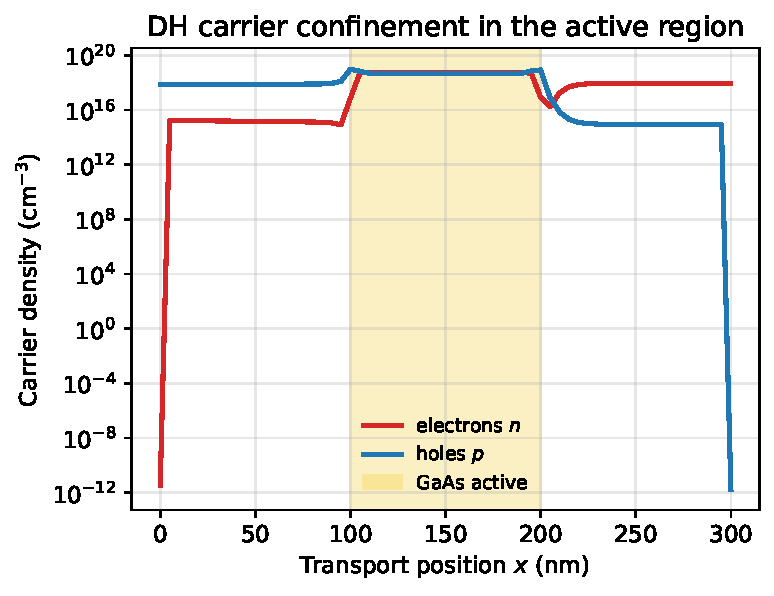
\includegraphics[width=\columnwidth]{fig_dh_confinement.pdf}
\caption{Carrier confinement in the GaAs/AlGaAs double-heterostructure LED
(shaded: GaAs active region). Heterojunction band offsets confine both electrons
and holes to the active region, where they overlap and recombine radiatively.}
\label{fig:dhconf}
\end{figure}

\begin{figure}[!t]
\centering
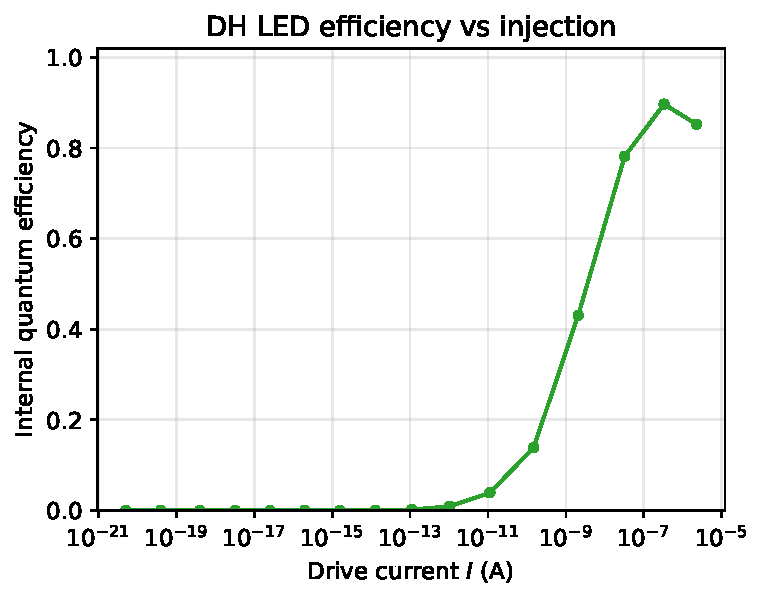
\includegraphics[width=\columnwidth]{fig_dh_iqe.pdf}
\caption{Internal quantum efficiency of the double-heterostructure LED versus
drive current. Carrier confinement raises the peak IQE to $0.90$, versus $0.53$
for the GaAs homojunction (Fig.~\ref{fig:gaasiqe}).}
\label{fig:dhiqe}
\end{figure}

\subsection{Discussion}
Three features make the model suitable for nano-photonic device design. First, the
radiative rate shares the terminal-current scale, so $qR_{\mathrm{rad}}$ is exactly
the radiative part of the current and the optical output cannot drift from the
electrical solution. Second, all corrections are opt-in and vanish in their bulk
limits, so a single code path spans a simple homojunction and a fully-corrected DH
quantum device. Third, the analytic Jacobian is preserved by every correction,
keeping the solve robust. The present optical model reports internal quantum
efficiency and the active-gap emission line; extraction efficiency, spectral
broadening and multi-quantum-well active regions ($k\!\cdot\!p$ subbands) are
natural extensions.

\section{Conclusion}
We have presented an open-source finite-element drift-diffusion solver for
direct-gap III--V light-emitting diodes that couples carrier transport to
bimolecular radiative recombination and a current-consistent optical
post-processor, with heterojunction, Schr\"odinger--Poisson and Fermi--Dirac
corrections on the same mesh. The GaAs LED characteristics are validated against
analytic physics; material selection tunes the emission from $873$~nm (GaAs) to
$366$~nm (GaN); and a GaAs/AlGaAs double heterostructure raises the peak internal
quantum efficiency from $0.53$ to $0.90$ by confining carriers to the active
region. The tool is a compact, physically transparent platform for the design of
nanoscale direct-gap emitters.

\section*{Software and Reproducibility}
The solver and the example scripts that generated every figure are open-source
(MIT licence) and require only a structured mesh built by the bundled generator.

\begin{thebibliography}{1}
\bibitem{schubert} E.~F.~Schubert, \emph{Light-Emitting Diodes}, 2nd~ed.
Cambridge, U.K.: Cambridge Univ. Press, 2006.
\bibitem{kroemer} H.~Kroemer, ``A proposed class of heterojunction injection
lasers,'' \emph{Proc. IEEE}, vol.~51, no.~12, pp.~1782--1783, 1963.
\bibitem{caseypanish} H.~C.~Casey and M.~B.~Panish, \emph{Heterostructure Lasers}.
New York: Academic Press, 1978.
\bibitem{selberherr} S.~Selberherr, \emph{Analysis and Simulation of Semiconductor
Devices}. Vienna: Springer-Verlag, 1984.
\bibitem{demari} A.~De Mari, ``An accurate numerical steady-state one-dimensional
solution of the p-n junction,'' \emph{Solid-State Electron.}, vol.~11, no.~1,
pp.~33--58, 1968.
\bibitem{sze} S.~M.~Sze and K.~K.~Ng, \emph{Physics of Semiconductor Devices},
3rd~ed. Hoboken, NJ: Wiley, 2007.
\bibitem{anderson} R.~L.~Anderson, ``Experiments on Ge--GaAs heterojunctions,''
\emph{Solid-State Electron.}, vol.~5, no.~5, pp.~341--351, 1962.
\end{thebibliography}

\end{document}
